\documentclass{article}

\usepackage{amsmath,amsthm,xcolor,graphicx}
\usepackage[pdftex]{hyperref}







\begin{document}

\def\imp{\Rightarrow}
\newcommand{\rstar}[1]{#1^*}
\newcommand{\rplus}[1]{#1^+}
\newcommand{\reqv}[1]{#1^\sim}
\newcommand{\toplus}{\rplus\to}
\newcommand{\tostar}{\rstar\to}
\newcommand{\tobeta}{\to_\beta}
\newcommand{\tobetaplus}{\to^+_\beta}
\newcommand{\tobetastar}{\to^*_\beta}
\newcommand{\tobetap}{\to_{p}}
\newcommand{\tobetapplus}{\to^+_{p}}
\newcommand{\tobetapstar}{\to^*_{p}}
\newcommand{\betaeqv}{\sim_\beta}
\newcommand{\toeqv}{\reqv\to}
\newcommand{\neglow}{\neg\,}

\newcommand{\diamg}[6]{
  \begin{matrix}
    #3 & #1 & #4 \\
    #2 &      & #2 \\
    #5 & #1 & #6
  \end{matrix}
}
\newcommand{\diam} [4] {
  \diamg{\to}{\downarrow}{#1}{#2}{#3}{#4}
}
\newcommand{\diamp} [4] {
  \diamg{\to_p}{\downarrow_p}{#1}{#2}{#3}{#4}
}

\newcommand{\indrule}[2]{\begin{array}{l} #1 \\ \hline #2\end{array}}
\newcommand{\ruleh}[2]{\begin{array}{c} #1 \\ \hline #2\end{array}}
\newcommand{\rulev}[2]{\begin{array}{l} #1 \\ \hline #2\end{array}}

\theoremstyle{definition} \newtheorem{definition}{Definition}[section]
\theoremstyle{definition} \newtheorem{theorem}{Theorem}[section]
\theoremstyle{definition} \newtheorem{lemma}{Lemma}[section]


\title{Lambda Calculus - Step by Step}
\author{Helmut Brandl}
\date{}


\maketitle

\tableofcontents

\section{Motivation}

This is a picture of David
Hilbert: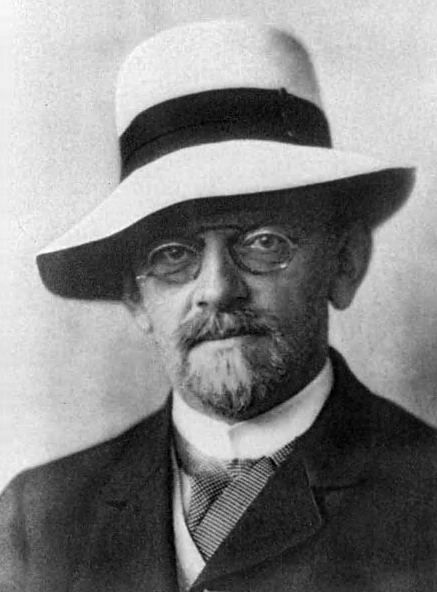
\includegraphics[scale=0.2,angle=90]{../img/hilbert.jpg} This is the text
which follows.


\section{Inductive Sets and Relations}


\begin{definition} The \emph{transitive closure} $\rplus{r}$ of a relation $r$ is
  defined by the rules
1.~$\rulev{r(a,b)}{\rplus{r}(a,b)}$,
2.~$\rulev{\rplus{r}(a,b) \\ r(b,c)}{\rplus{r}(a,c)}$
\end{definition}

\begin{definition} The \emph{reflexive transitive closure} $\rstar{r}$ of a relation $r$ is
  defined by the rules
1.~$\rulev{}{\rstar{r}(a,a)}$,
2.~$\rulev{\rstar{r}(a,b) \\ r(b,c)}{\rstar{r}(a,c)}$
\end{definition}

\begin{definition} The \emph{equivalence closure} $\reqv{r}$ of a relation $r$ is
  defined by the rules
  1.~$\rulev{}{\reqv{r}(a,a)}$,
  2.~$\rulev{\reqv{r}(a,b)
    \\ r(b,c)} {\reqv{r}(a,c)}$,
  3.~$\rulev{\reqv{r}(a,b) \\ r(c,b)} {\reqv{r}(a,c)}$
\end{definition}

\begin{theorem}
  All closures are increasing $r \subseteq r^c$, monotonic
  $r \subseteq s \imp r^c \subseteq s^c$ and idempotent $r^{cc} = r$. Proof
  e.g. for the reflexive transitive closure. TBD.
\end{theorem}

\begin{theorem}
A relation $s$ which satisfies $r \subseteq s \subseteq r^c$ has the same closure
as $r$ i.e. $r^c = s^c$. Proof:
  \begin{itemize}
  \item $r^c \subseteq s^c$ by monotonicity.
  \item $s^c \subseteq r^c$: $s^c \subseteq r^{cc}$ by
    monotonicity and then use idempotence to conclude $s^c \subseteq r^c$.
  \end{itemize}
\end{theorem}



Theorems: $\rplus{r}$ is transitive, $\rstar{r}$ is transitive, $\reqv{r}$ is
symmetric, $\rplus{r}\subseteq\rstar{r}$, $r$ reflexive $\imp \rplus{r} =
\rstar{r}$.


\begin{definition}
  $a$ is a \emph{terminal element} of the relation $\to$ if it has no
  successor i.e. $\forall b: \neglow a \to b$.
\end{definition}

\begin{definition}
  $a$ is a \emph{terminating element} of the relation $\to$ if there is a path
  to a terminal element $b$ i.e. $a \tostar b$.
\end{definition}

\begin{definition}
A relation $\to$ is a \emph{diamond} if for all $a$, $b$ and $c$ there exists a $d$
such that
$
  \begin{matrix}
    a & \to & b \\
    \downarrow & & \downarrow \\
    c & \to & \exists d
  \end{matrix}
$
\end{definition}


\begin{definition}
  A relation $r$ is \emph{confluent} if $\rstar{r}$ is a diamond.
\end{definition}

\begin{theorem} In a confluent relation $r$ all two $r$-equivalent elements
  meet at some common element
  $
  \begin{matrix}
    a & \reqv\to & b \\
    & \rstar\searrow & \downarrow_*\\
    & & \exists c
  \end{matrix}
  $.
  Proof by induction on $a\reqv\to b$.
  \begin{enumerate}

  \item $a = b$. Trivial. Take $c = a$.

  \item
    $\begin{matrix}
      a & \reqv\to & b & \to & c\\
      & \rstar\searrow & \downarrow_*  & & \downarrow_*\\
      & & d? & \rstar\to & e?
    \end{matrix}$.
    $d$ exists by induction hypothesis, $e$ exists by confluence.

  \item
    $
    \begin{matrix}
      a & \reqv\to & b & \gets & c\\
      & \rstar\searrow & \downarrow_*  & & \downarrow_*\\
      & & d? & \rstar\to & e?
    \end{matrix}
    $.
    $d$ exists by induction hypothesis, $e$ exists by confluence.
  \end{enumerate}
\end{theorem}

Definition: $a$ is a terminal element of $r$ if $\neg r(a,b)$ for all $b$.

Definition: Set $\overline T$ of terminating elements of a relation $r$:
$\rulev{a\in T}{a\in \overline T}$, $\rulev{r(a,b) \\ b\in\overline T}{a\in
  \overline T}$ where $T$ is the set of terminal elements. By definition: For
all terminating elements $a$ there is a terminal element $b$ with $\rstar
r(a,b)$.

Theorem: In a confluent relation all terminating elements have a unique
terminal element. Proof: Suppose there are two terminal elements $b$ and $c$
for the terminating element $a$. By definition there must be a $d$ such that
$\begin{matrix} a & \tostar & b \\
  \downarrow_* & & \downarrow_* \\
  c & \tostar & d
\end{matrix}$
which contradicts the assumption that $b$ and $c$ are terminal.


Theorem: In a confluent relation $r$ two $r$-equivalent terminating elements have the same
terminal element.
Proof: Assume $a \reqv\to b$ and $a \to_* c$ and $b \to_* d$
where $c$ and $d$ are different terminal elements. Prove by induction on $a
\reqv\to b$. Case (a): $a=b$. By the previous theorem the terminal element
must be unique. Contradiction. Case (b): $a \reqv\to b$ and $b \to c$. By
induction hypothesis $a$ and $b$ must have the same terminal element.

Theorem: The reflexive transitive closure of a diamond is a diamond (stripe
lemma).
Proof:
\begin{itemize}
\item Lemma: Let $\to$ be a diamond. Then
$\begin{matrix}
a & \to_* & b \\
\downarrow & & \downarrow \\
c & \to_* & \exists d
  \end{matrix}$.
Proof by induction on $a \to_* b$.
\begin{itemize}
\item Case (a): $a = b$. Trivial, take $d=c$.
\item Case (b):
$\begin{matrix}
a & \to_* & b & \to & c\\
\downarrow & & \downarrow & & \downarrow\\
d & \to_* & e? & \to & f?
\end{matrix}$. $e$ exists by the induction hypothesis, $f$ exists because
$\to$ is a diamond.
\end{itemize}

\item Theorem:  Let $\to$ be a diamond. Then
$\begin{matrix}
a & \to_* & b \\
\downarrow_* & & \downarrow_* \\
c & \to_* & \exists d
  \end{matrix}$. Proof by induction on $a \to_* c$.
\begin{itemize}
\item Case (a): $a = b$. Trivial, take $d=c$.
\item Case (b):
$\begin{matrix}
a & \to_* & b\\
\downarrow_* & & \downarrow_* \\
c & \to_* & e?  \\
\downarrow & & \downarrow \\
d & \to_* & f?
\end{matrix}$. $e$ exists by induction hypothesis, $f$ exists by the previous lemma.
\end{itemize}
\end{itemize}



\section{Lambda Terms}

\begin{definition}
  Let $x$ range over a countably infinite set of variable names then the set
  of lambda terms is defined by the grammar $$t ::= x \mid t t \mid \lambda x. t$$.
\end{definition}

A lambda term is either a variable $x$, an application $a b$ (the term $a$
applied to the term $b$) or an abstraction $\lambda x.a$.

We use the convention that application is left associative i.e. $a b c$ is
parsed as $(a b) c$.

Nested lambda abstractions $\lambda x. \lambda y. \ldots . t$ are parsed as
$\lambda x. (\lambda y. \ldots . t)$ and abbreviated as $\lambda x y \ldots . t$

\begin{definition}
  The set of free variables $FV(t)$ of a lambda term $t$ is defined by
  $$FV(t) :=
  \begin{cases} FV(x) &= \{x\} \\
     FV(a b) &= FV(a) \cup FV(b) \\
     FV(\lambda x. t) &= FV(t) - \{x\}
   \end{cases}
   $$
\end{definition}

The variable $x$ in the term $t$ of the abstraction $\lambda x.t$ is a bound
variable. Bound variables can be renamed arbitrarily. We consider terms equal
which have just different namings of bound variables. E.g. the term $\lambda
x.x$ and $\lambda y.y$ are equal.

\begin{definition}
  The variable substitution $a[x:=t]$ is defined by
  $$a[x:=t]~:=
  \begin{cases} x[x:=t]  &:= t \\
    y[x:=t] &:= y \quad \text{for}\quad x \ne y \\
    (a b)[x:=t] &:= a[x:=t] \, b[x:=t] \\
    (\lambda y.a)[x:=t]  &:= \lambda y. a[x:=t] \quad\text{for}\quad x \ne y
    \land y \notin FV(t)
   \end{cases}
   $$
\end{definition}

Note: The condition on the last line is no restriction because we can always
rename the bound variable $y$ to a fresh variable $z$ different from $x$ and
not occuring free in $t$ since there are infinitely many variables available.

Two subsequent substitutions do not commute. The terms $a[x:=b][y:=c]$ and
$a[y:=c][x:=b]$ are different in general even if $x \ne y$ and
$x \notin FV(c)$. Reason: Neither $a[x:=b][y:=c]$ nor $a[y:=c]$ do contain any
$y$. But $b$ might contain $y$ and therefore $a[y:=c][x:=b]$ might contain
$y$. In order to make the swapping correct we have to do the substitution
$b[y:=c]$ before substituting the variable $x$ by $b$.

\begin{theorem} Substitution lemma: Let $x \ne y$ and $x \notin
  FV(c)$. Then $$a[x:=b][y:=c] = a[y:=c]\big[x:= b[y:=c]\big]$$. Proof by
  induction on the structure of $a$. We use the abbreviations
  $$\begin{array}{ll}
      s_1(a) &:= a[x:=b][y:=c] \\
      s_2(a) &:= a[y:=c]\big[x:=b[y:=c]\big]
    \end{array}$$.
  \begin{enumerate}
  \item $a$ is a variable. Lets call it $z$. To prove $s_1(z) = s_2(z)$
    \begin{itemize}
    \item $z \ne x \land z \ne y$: $s_1(z) = z = s_2(z)$
    \item $z = x \land z \ne y$: $s_1(z) = b[y:=c] = s_2(z)$
    \item $z \ne x \land z = y$: $s_1(z) = c = s_2(z)$
    \end{itemize}
  \item $a$ is the application $t u$.
    $$\begin{array}{llll}
        s_1(t u) &=& s_1(t) s_1(u) & \text{definition of substitution}\\
       &=& s_2(t) s_2(u) & \text{induction hypothesis}\\
        &=& s_2(t u) & \text{definition of substitution}
      \end{array}$$
      with the abbreviations $s_1(v) := v[x:=b][y:=c]$ and $s_2(v) :=
      v[y:=c][x:=b[y:=c]]$.
    \item $a$ is the abstraction $\lambda z.t$.
    $$\begin{array}{llll}
        s_1(\lambda z. t) &=& \lambda z. s_1(t)  & \text{definition of substitution}\\
       &=& \lambda z. s_2(t) & \text{induction hypothesis}\\
        &=& s_2(\lambda z.t) & \text{definition of substitution}
      \end{array}$$
      with appropriate renaming of the bound variable $z$ in order to avoid
      variable capture.
  \end{enumerate}
\end{theorem}





\begin{definition} \emph{Beta reduction} $\tobeta$ is a relation defined over lambda
  terms by the rules
  \begin{enumerate}
  \item $(\lambda x.a) b \tobeta a[x := b]$
  \item $\rulev{a\tobeta b}{a c \tobeta b c}$
  \item $\rulev{b\tobeta c}{a b \tobeta a c}$
  \item $\rulev{a \tobeta b}{\lambda x.a \tobeta \lambda x.b}$
  \end{enumerate}
\end{definition}




\begin{theorem}
  $\tobetastar$ preserves abstraction
  %---------------------------
  i.e. $a \tobetastar b \imp \lambda x.a \tobetastar \lambda x.b$.
  Proof by induction on $a \tobetastar b$.
  \begin{enumerate}
  \item Goal $a \tobetastar a \imp \lambda x.a \tobetastar \lambda
    x.a$. Trivial by reflexivity of $\tobetastar$.
    \item
      Goal $a \tobetastar c \imp \lambda x.a \tobetastar \lambda x.c$.
      Premises $a \tobetastar b, b \tobeta c$.
      Induction hypothesis $\lambda x.a \tobetastar \lambda x.b$.
      We get $\lambda x.b \tobeta \lambda x.c$ by rule 2 of $\tobeta$ and
      the goal by rule 2 of reflexive transitive closure.
  \end{enumerate}
\end{theorem}


\begin{lemma}
  Basic application preservation lemma of $\tobetastar$:
  $b \tobetastar c  \imp a b \tobetastar a c$.
  %------------------------------------------
  Proof by induction on $b \tobetastar c$.
  \begin{enumerate}
  \item
    Trivial by reflexivity of the closure.
  \item
    Goal $b \tobetastar d  \imp a b \tobetastar a d$.
    Premises $b \tobetastar c$ and $c \tobeta d$.
    Induction hypothesis $b \tobetastar c  \imp a b \tobetastar a c$.
    From $c \tobeta d$ we get $a c \tobeta a d$ by rule 3 of beta reduction
    and $a b \tobetastar a d$ by rule 2 of the reflexive transitive closure.
  \end{enumerate}
\end{lemma}



\begin{theorem}
  $\tobetastar$ preserves application
  i.e. $a \tobetastar b \land c \tobetastar d \imp a c \tobetastar b d$.
  %----------------------------------------------------
  Proof by induction on $a \tobetastar b$.
  \begin{enumerate}
  \item
    Goal $a \tobetastar a \land c \tobetastar d \imp a c \tobetastar a d$.
    By previous lemma.
  \item
    Goal $a \tobetastar e \land c \tobetastar d \imp a c \tobetastar e d$.
    Premises $a \tobetastar b$ and $b \tobeta e$.
    Induction hypothesis $a \tobetastar b \land c \tobetastar d \imp
    a c\tobetastar b d$.
    From $b \tobeta e$ be get $b d \tobeta e d$ by rule 2 of beta reduction
    and $a c \tobetastar e d$ by rule 2 of the reflexive transitive closure.
  \end{enumerate}
\end{theorem}



\begin{theorem}
  $\tobetastar$ preserves reduction
  i.e. $a \tobetastar b \land c \tobetastar d \imp
  (\lambda x.a) c \tobetastar b[x:=d]$.
  %----------------------------------------------------
  Proof similar to the proof of the preservation of application in two steps
  by first proving a lemma where only $c$ is reduced to $d$ and then the
  complete theorem.
\end{theorem}






\section{Church Rosser (Confluence)}

\begin{definition}
  % -------------------------------------------------------
  \emph{Parallel beta reduction} $\tobetap$ is a relation
  defined over lambda terms by the rules
  % -------------------------------------------------------
  \begin{enumerate}
  \item $a \tobetap a$
  \item $\rulev{a \tobetap b} {\lambda x.a \tobetap \lambda x.b}$
  \item $\rulev{a\tobetap c \\ b \tobetap d}{a b \tobeta c d}$
  \item $\rulev{a\tobetap c \\ b \tobetap d}{(\lambda x.a) b \tobetap c[x := d]}$
  \end{enumerate}
\end{definition}

\begin{lemma}
  Beta reduction is a subset of parallel beta reduction i.e.
  %---------------------------------------
  $a \tobeta b \imp a \tobetap b$.
  Proof by induction on $a \tobeta b$. Trivial because each rule of $\tobeta$
  is a special case of some rule of $\tobetap$.
\end{lemma}


\begin{lemma}
  Parallel beta reduction is a subset of the reflexive transitive closure of
  beta reduction i.e.
  %---------------------------------------
  $a \tobetap b \imp a \tobetastar b$.
  Proof by induction on $a \tobetap b$.
  \begin{enumerate}
  \item
    Trivial by reflexivity.
  \item
    Goal $
    (\lambda x.a) \tobetap \lambda x.b  \imp
    (\lambda x.a) \tobetastar \lambda x.b$.
    Premise $a \tobetap b$.
    Induction hypothesis $a \tobetastar b$.
    Since $\tobetastar$ preserves abstraction (theorem of the previous
    chapter) we can conclude the goal.
  \item
    Goal $a c \tobetap b d \imp a c \tobetastar b d$.
    Premises $a \tobetap b$ and $c \tobetap d$.
    Induction hypotheses $a \tobetap b \imp a \tobetastar b$ and
    $c \tobetap d \imp c \tobetastar d$.
    Since $\tobetastar$ preserves application we can conclude the goal $a c
    \tobetastar b d$.
  \item
    Goal $(\lambda x.a) c \tobetap b[x:=d] \imp
    (\lambda x.a) c \tobetastar b[x:=d]$.
    Premises $a \tobetap b$ and $c \tobetap d$.
    Induction hypotheses $a \tobetap b \imp a \tobetastar b$ and
    $c \tobetap d \imp c \tobetastar d$.
    Since $\tobetastar$ preserves reduction we can conclude the goal $(\lambda x.a) c
    \tobetastar b[x:=d]$.
  \end{enumerate}
\end{lemma}



\begin{theorem}
  Parallel beta reduction is between beta reduction and its transitive closure
  i.e. $(\tobeta) \subseteq (\tobetap) \subseteq (\tobetastar)$.
  %----------------------------------------------------------
  Proof by the previous two lemmas.
\end{theorem}




In order to prove that $\tobetap$ is a diamond we need some lemmas.

\begin{lemma}
  Parallel beta reduction preserves abstraction i.e.
  $\lambda x.a \tobetap c \imp \exists b : a \tobetap b \land c = \lambda
  x.b$. Proof by induction on $\tobetap$.
  \begin{enumerate}
  \item $c = \lambda x.a$. Trivial. Take $b = a$.
  \item $\lambda x.a \tobetap \lambda x.b$ with $a \tobetap b$. Trivial. Take $b$.
  \item The case $\lambda x.a = t u$ is syntactically impossible. Abstraction
    and application are different.
  \item The case $\lambda x.a = (\lambda x.u) v$ is syntactically
    impossible. Abstraction and application are different.
  \end{enumerate}
\end{lemma}


\begin{lemma}
  Basic compatibility of substitution and parallel reduction.
  $t \tobetap u \imp a[x := t] \tobetap a[x := u]$. Proof by induction on the
  structure of $a$.
  \begin{enumerate}
  \item $a$ is a variable. Goal $z[x := t] \tobetap z[x := u]$. Case $z=x$
    is satisfied because of the assumption $t \tobetap u$. Case $z\ne x$ is
    satisfied by reflexivity $z \tobetap z$.
  \item
    $a$ is an application $b\, c$.
    Goal $(b c)[x:=t] \tobetap (b c)[x:=u]$
    $$
    \begin{array}{llll}
      (b c)[x:=t] &=& b[x:=t]\, c[x:=t] &              \text{definition of substitution}\\
                      &\tobetap & b[x:=u]\, c[x:=u] & \text{ind hypo + rule 3} \\
                      &=& (b c)[x:=u] &                       \text{definition of substitution}
    \end{array}
    $$
  \item
    $a$ is an abstraction $\lambda y.b$.
    Goal $(\lambda y.b)[x:=t] \tobetap (\lambda y.b)[x:=u]$.
    $$
    \begin{array}{llll}
      (\lambda y.b)[x:=t] &=& \lambda y. b[x:=t]  &\text{definition of substitution}\\
      &\tobetap & \lambda y.b[x:=u] &\text{ind hypo + rule 2} \\
      &=& (\lambda y.b)[x:=u] & \text{definition of substitution}
    \end{array}
    $$
  \end{enumerate}
\end{lemma}


\begin{lemma}
  Full compatibility of substitution and parallel reduction.
  % a -> c and b -> d  =>  a[x:=b] -> c[x:=d]
  % ----------------------------------
  $a \tobetap c \land b \tobetap d  \imp a[x := b] \tobetap c[x := d]$. Proof
  by induction on $a \tobetap c $.
  \begin{enumerate}
  \item
    $a=c$. Prove by the previous lemma.
  \item
    Goal $(\lambda y.a) [x := b] \tobetap (\lambda y.c) [x := d]$.
    Premise $a \tobetap c$. Induction
    hypothesis $a[x := b] \tobetap c[x := d]$
    $$
    \begin{array}{llll}
      (\lambda y.a)[x := b]  &=& \lambda y.a [x := b] &\text{definition substitution} \\
                             &\tobetap& \lambda y.c[x := d]  &\text{induction hypo + rule 2} \\
                             &=& (\lambda y.c)[x := d]           &\text{definition substitution}
    \end{array}
    $$.
  \item
    Goal $(a e) [x := b] \tobetap (c f) [x := d]$.
    Premises $a\tobetap c, e\tobetap f$.
    Induction hypotheses
      $a[x := b] \tobetap c[x := d],
       e[x := b] \tobetap f[x := d]$
    $$
    \begin{array}{llll}
      (a e)[x := b]  &=& a[x := b]\, e[x := b] &\text{definition substitution}\\
                     &\tobetap& c[x := d] \, f[x := d] &\text{induction hypo + rule 3} \\
                     &=& (c f)[x := d] &\text{definition substitution}
    \end{array}
    $$.
  \item
    Goal $\big((\lambda y.a) c\big) [x := b] \tobetap \big(e[y:=f]\big)[x := d]$.
    Premises $a \tobetap e, c \tobetap f$.
    Induction hypotheses
      $a[x:=b] \tobetap e[x := d],
        c[x:=b]  \tobetap f[x := d]$
    $$
    \begin{array}{llll}
      ((\lambda y.a) c)[x := b]  &=& (\lambda y.a[x := b])\, c[x := b] &
                                                                         \text{definition substitution}\\
                     &\tobetap& e[x := d]\big[y:=f[x := d]\big] &
                                                                  \text{induction hypo + rule 4} \\
                     &=& \big(e[y:=f]\big)[x := d] &
                                                                  \text{substitution
                                                           swap lemma}
    \end{array}
    $$
  \end{enumerate}
  $\qed$
\end{lemma}





\begin{theorem}
  Parallel reduction $\tobetap$ is a diamond i.e.
  %------------------------------------
  $\begin{matrix}
    a & \tobetap & b \\
    \downarrow_p & & \downarrow_p \\
    c & \tobetap & \exists d
  \end{matrix}
  $.
  Proof by induction on $a \tobetap b$.
  \begin{enumerate}
  \item
    Trivial reflexive case.
    $\diamp
    {a} {a}
    {c} {c}
    $

  \item Goal
    $\diamp
    {\lambda x.a} {\lambda x.b}
    {\lambda x.c} {?}$.
    Parallel reduction preserves abstraction. Therefore the specific
    $\lambda x.c$ instead of the more general $c$.
    The premises $a\tobetap b, a \tobetap c$ and the induction hypothesis
    guarantees the existence of a $d$ such that $\lambda x.d$ is the element
    to fill the gap.

  \item
    Goal $\diamp {a e} {b f} {c}  {?}$. Premises $a \tobetap b, e \tobetap f$.
    Proof by subinduction on $a e \tobetap c$.

    \begin{enumerate}
    \item Trivial reflexive case.
    \item Syntactically impossible
    \item
      Goal $\diamp {a e} {b f} {g h} {?}$.

      The premises $a \tobetap b, a \tobetap g, e \tobetap f, e \tobetap h$
      with the corresponding induction hypotheses guarantee the existence of
      two element $k$ and $m$ so that $ k m$ can fill the missing element in
      the goal.

    \item
      Goal $\diamp {(\lambda x.a) e} {(\lambda x.b) f} {c[x:=g]} {?}$.
      Parallel reduction preserves abstraction. Therefore the specific
      $\lambda x.b$ in the upper right corner.
      The premises $a \tobetap b, a \tobetap c, e \tobetap f, e \tobetap g$
      and the corresponding induction hypotheses guarantee the existence of
      two elements $d$ and $h$ so that $d[x:=h]$ fills the missing element
      in the goal.
    \end{enumerate}

  \item
    Goal $\diamp {(\lambda x.a) e} {b[x:=f]} {c} {?}$. Premises $a \tobetap b, e \tobetap f$.
    Proof by subinduction on $(\lambda x.a) e \tobetap c$.
    \begin{enumerate}
    \item Trivial reflexive case.
    \item Syntactically impossible
    \item Mirror image of case 3d, just flipped at the northwest-southeast diagonal.
    \item
      Goal $\diamp {(\lambda x.a) e} {b[x:=f]} {c[x:=g]} {?}$
      The premises $a \tobetap b, a \tobetap c, e \tobetap f, e \tobetap g$
      and the corresponding induction hypotheses guarantee the existence of
      two elements $d$ and $h$ so that $d[x:=h]$ fills the missing element
      in the goal.
    \end{enumerate}

  \end{enumerate}
  $\qed$
\end{theorem}


\begin{theorem}
  Beta reduction is confluent.
  %--------------------
  Proof: With the parallel beta reduction$\tobetap$ we have found a diamond
  relation between beta reduction $\tobeta$ and its transitive closure
  $\tobetastar$. According to the confluence theorems of the chapter
  ``Inductive Sets and Relations'' this is sufficient to prove the confluence
  of beta reduction.
\end{theorem}

\section{Reduction Strategies}

\section{Computations}

\section{Undecidability}


\begin{thebibliography}{99}

\bibitem{church1936} Church, A. (1936). An unsolvable problem of elementary number theory, American
Journal of Mathematics 58, pp. 354–363.

\bibitem{chuchrosser1936} Church, A., Rosser, J. B.: Some Properties of Conversion, Trans. Amer. Math. Soc., 39, 1936, 472–482.


\bibitem{goedel1931} Kurt Gödel (1931). Über formal unentscheidbare Sätze der
  Principia Mathematica und verwandter Systeme I, Monatshefte für Mathematik
  und Physik, vol. 38 (1931), pp. 173-198.

\bibitem{schoenfinkel1924} Schönfinkel, M. (1924). Über die Bausteine der mathematische Logik, Mathematische
Annalen 92, pp. 305–316.

\bibitem{turing1936} Turing, A.M. (1936/7). On computable numbers, with an application to the
Entscheidungsproblem, Proceedings of the London Mathematical Society
42, pp. 230–265.

\end{thebibliography}


\end{document}
